\documentclass[10pt]{article}

\usepackage{akteach}
\usepackage{amsmath}
\usepackage{amsfonts}
\usepackage{amssymb}
\usepackage{amsthm}
\usepackage{float}
\usepackage{algpseudocode}
\usepackage[all]{xy}


\newcommand{\C}{\mathbb{C}}
\newcommand{\Q}{\mathbb{Q}}
\newcommand{\K}{\mathbb{K}}
\newcommand{\proj}{\mathbb{P}}
\newcommand{\T}{\mathbb{T}}
\newcommand{\F}{\mathbb{F}}
\newcommand{\Z}{\mathbb{Z}}
\newcommand{\N}{\mathbb{N}}
\newcommand{\set}{\mathcal{S}}
\newcommand{\cp}{\mathbb{C}P}
\newcommand{\A}{\mathcal{A}}
\newcommand{\BB}{\mathcal{B}}
\newcommand{\CC}{\mathcal{C}}
\newcommand{\NN}{\mathcal{N}}
\newcommand{\LL}{\mathcal{L}}
\newcommand{\MM}{\mathcal{M}}
\newcommand{\E}{\mathcal{E}}
\newcommand{\FF}{\mathcal{F}}
\newcommand{\G}{\mathcal{G}}
\newcommand{\eps}{\varepsilon}
\newcommand{\Hom}{\text{Hom}}
\newcommand{\Div}{\text{div}}
\newcommand{\Res}{\text{Res}}
\newcommand{\ord}{\text{ord}}
\newcommand{\Deg}{\text{deg}}
\newcommand{\mult}{\text{mult}}

\newcommand{\id}{\text{id}}
\newcommand{\Tr}{\text{Tr}}
\newcommand{\ad}{\text{ad}}
\newcommand{\Ad}{\text{Ad}}
\newcommand{\Aut}{\text{Aut}}
\newcommand{\der}{\text{der}}
\newcommand{\GL}{\text{GL}}
\newcommand{\gl}{\mathfrak{gl}}
\newcommand{\rad}{\mathfrak{rad}}
\newcommand{\inhook}{\hookrightarrow}
\newcommand{\sgn}{\text{sign}}

\begin{document}

\akteachheader{Numerical Analysis (CS 450)}%
{Homework Set 4, Bill Karr}

\akteachprobhead{%
  Problem 1: Optimization Theory (20 points)
}

\begin{itemize}

\item[(a)] Prove that any local minimum of a convex function $f$ on a convex set $ \set \subseteq \R^n $ is a global minimum of $f$ on $\set$.

\begin{proof}
Suppose $ x \in \set $ is a local minimum of $f$ but not a global minimum. Then, choose $ y \in \set $ with $ f(y) < f(x) $. Since $f$ is convex, then for any $ s,t \in (0,1) $ with $ s + t = 1 $, we have $$
f(sx + ty) \leq sf(x) + tf(y) < sf(x) + tf(x) = (s + t)f(x) = f(x).
$$ So, $ f $ is smaller than $f(x)$ on the whole open line segment between $x$ and $y$. Therefore, $f(x)$ is \textit{not} a local minimum, a contradiction. \end{proof}

\item[(b)] Let $ f : \R^n \to \R $ and $ g : \R^n \to \R^m $. Consider the optimization problem $$
\min_{x} f(x) \text{ subject to } g(x) = 0.
$$ Show that the Hessian of the \textit{Lagrangian function} $ \LL : \R^{n+m} \to \R $ $$
\LL(y) = \LL(x,\lambda) = f(x) + \lambda^T g(x)
$$ is given by $$
H_\LL (x,\lambda) = \begin{bmatrix}
H_f(x) + \sum_{i = 1}^m \lambda_i H_{g_i}(x) & J^T_{g}(x) \\
J_{g}(x) & 0
\end{bmatrix}.
$$

\begin{proof}
We need only compute all of the second partial derivatives. $$
\frac{\partial^2 \LL}{\partial x_i \partial x_j}
= \frac{\partial^2 f}{\partial x_i \partial x_j} + \sum_{k=1}^m \lambda_k \frac{\partial^2 g_k}{\partial x_i \partial x_j} = 
(H_f(x))_{ij} + \sum_{k = 1}^m \lambda_k (H_{g_k})_{ij},
$$ $$
\frac{\partial^2 \LL}{\partial x_i \partial \lambda_j}
= \frac{\partial g_j}{\partial x_i} = ( J_{g}(x) )_{ji},
$$ $$
\frac{\partial^2 \LL}{\partial \lambda_i \partial x_j}
= \frac{\partial}{\partial \lambda_i} \left( \frac{\partial f}{\partial x_j} + \lambda^T \frac{\partial g}{\partial x_j} \right) = \frac{\partial g_i}{\partial x_j} = (J_g(x))_{ij},
$$ and finally $$
\frac{\partial^2 \LL}{\partial \lambda_i \partial \lambda_j} = 0
$$ since $ \LL $ only depends linearly on the $\lambda_i$. Thus, putting these terms together in a matrix, we see that $$
H_\LL (x,\lambda) = \begin{bmatrix}
H_f(x) + \sum_{k = 1}^m \lambda_k H_{g_k}(x) & J^T_{g}(x) \\
J_{g}(x) & 0
\end{bmatrix}.
$$ \end{proof}

\item[(c)] Prove that $ H_\LL(x,\lambda) $ cannot be positive definite. 

\begin{proof}
For any $ \beta \in \R^m \setminus \{ 0 \} $, notice that $$
\begin{bmatrix}
0 \\
\beta
\end{bmatrix}^T
\begin{bmatrix}
H_f(x) + \sum_{k = 1}^m \lambda_k H_{g_k}(x) & J^T_{g}(x) \\
J_{g}(x) & 0
\end{bmatrix}
\begin{bmatrix}
0 \\
\beta
\end{bmatrix} =
\begin{bmatrix} \beta^T J_g(x) & 0 \end{bmatrix}  \begin{bmatrix}
0 \\
\beta
\end{bmatrix} = 0
$$ Therefore, we can find nonzero vectors $ v \in \R^{n+m} $ so that $ v^T H_\LL(x,\lambda) v \not > 0 $, i.e. $ H_{\LL}(x,\lambda) $ is not positive definite.
\end{proof}

\item[(d)] What does the non-positive-definiteness of $ H_\LL(x,\lambda) $ mean for the solution of the problem $ \nabla \LL(x,\lambda) = 0 $?

\begin{proof}[Solution] It means that if we find a critical point of $\LL$, i.e. $ (x,\lambda) $ with $ \nabla \LL(x,\lambda) = 0 $, there is no guarantee that it will be an absolute minimum because $ \LL $ is not convex.
\end{proof}

\end{itemize}

\akteachprobhead{%
  Problem 2: Optimization on quadratic forms (20 points)
}

\begin{itemize}
\item[(a)] Provide an analytic expression for the gradient $ \nabla f $ and the Hessian $ H_f $.

\begin{proof}[Solution]
If $ f(x_1, ... , x_n) = \frac{1}{2} \sum_{i,j = 1}^n x_i A_{ij} x_j - \sum_{i = 1}^n x_i b_i + c $, then $$
\frac{\partial f}{\partial x_k} = \frac{1}{2} \sum_{i,j = 1}^n ( \delta_{ik} A_{ij} x_j + x_i A_{ij} \delta_{jk} ) - b_k = \frac{1}{2} \sum_{i = 1}^n ( A_{ki} x_i + A_{ik} x_i ) - b_k = \sum_{i = 1}^n A_{ki} x_i - b_k
$$ Thus, $ \nabla f(x) = Ax - b $.

In addition, $$
\frac{\partial^2 f}{\partial x_k \partial x_m} = A_{km}.
$$ Thus, $ H_f = A $.
\end{proof}

\item[(b)] At what point does $f$ attain a minimum?

\begin{proof}[Solution]
Since $A$ is symmetric and positive-definite, $f$ is convex and achieves its minimum at any critical point. Thus, when $$
\nabla f(x) = Ax - b = 0 \Rightarrow x = A^{-1} b,
$$ $f$ achieves its minimum.
\end{proof}

\item[(c)] Show that Newton's method for finding the minimum converges in one iteration from any starting point, $x_0$, by showing that the error after one step, $ e_1 = x_1 - x^* $, is zero.

\begin{proof}
Since $ H_f = A $ and $ \nabla f(x) = Ax - b $, then using Newton's method starting with $ x_0 \in \R^n $, we obtain $$
x_1 = x_0 - H_f(x_0)^{-1} \nabla f(x_0) = x_0 - A^{-1}( Ax_0 - b ) = x_0 - x_0 + A^{-1} b = A^{-1} b
$$ which is the minimum point of $f$. Therefore, Newton's method converges after one iteration.
\end{proof}

\item[(d)] Show that one step of steepest descend (for this function) can be written as $$
x_1 = x_0 + \frac{r^T r}{r^T A r} r
$$ where $ r = b - Ax $. What happens to the error after one step if the initial error, $ e_0 = x_0 - x^* $, is an eigenvector of $A$.

\begin{proof}
For the steepest descend method, we let $ r = -\nabla f(x_0) = b - Ax_0 $ and choose $ \alpha \in \R $ to minimize $ f(x_0 + \alpha r ) $. Then, $ x_1 = x_0 + \alpha r $.

Notice that $ \frac{d}{d \alpha} f(x_0 + \alpha r) = r^T \nabla f(x_0 + \alpha r) $. Thus, $ \frac{d}{d \alpha} f(x_0 + \alpha r) = 0 $ when $$
r^T ( A(x_0 + \alpha r) - b ) = 0 \Rightarrow r^T(Ax_0 - b) + \alpha r^T A r = 0 \Rightarrow \alpha = \frac{r^T r}{r^T A r}.
$$ We conclude that $$
x_1 = x_0 + \frac{r^T r}{r^T A r} r.
$$

If $ e_0 = x_0 - x^* = x_0 - A^{-1} b $ is an eigenvector with eigenvalue $ \lambda $, then $ r = - ( Ax_0 - b ) = -A(x_0 - A^{-1}b) = - \lambda(x_0 - x^*) $ is also an eigenvector of $A$ with the same eigenvalue and $ \alpha = r^T r/(r^T A r) = \frac{1}{\lambda} $. Thus, $$
x_1 = x_0 + \frac{r}{\lambda}.
$$ \end{proof}

\end{itemize}

\akteachprobhead{%
  Problem 3: Optimization and Nonlinear Data Fitting (20 points)
}

\begin{itemize}
\item[(a)] See \verb+cs450hw4p3.py+ for my code. The damped Newton's method finished after the fewest iterations and steepest descent took the longest. This makes sense since steepest descent has linear convergence and Newton's method already has quadratic convergence but the line search is only speeding that up by unsuring not to go too far at each step. Here are the plots for each of the three iterative methods with the four starting points:

\begin{figure}[H]
  \centering
    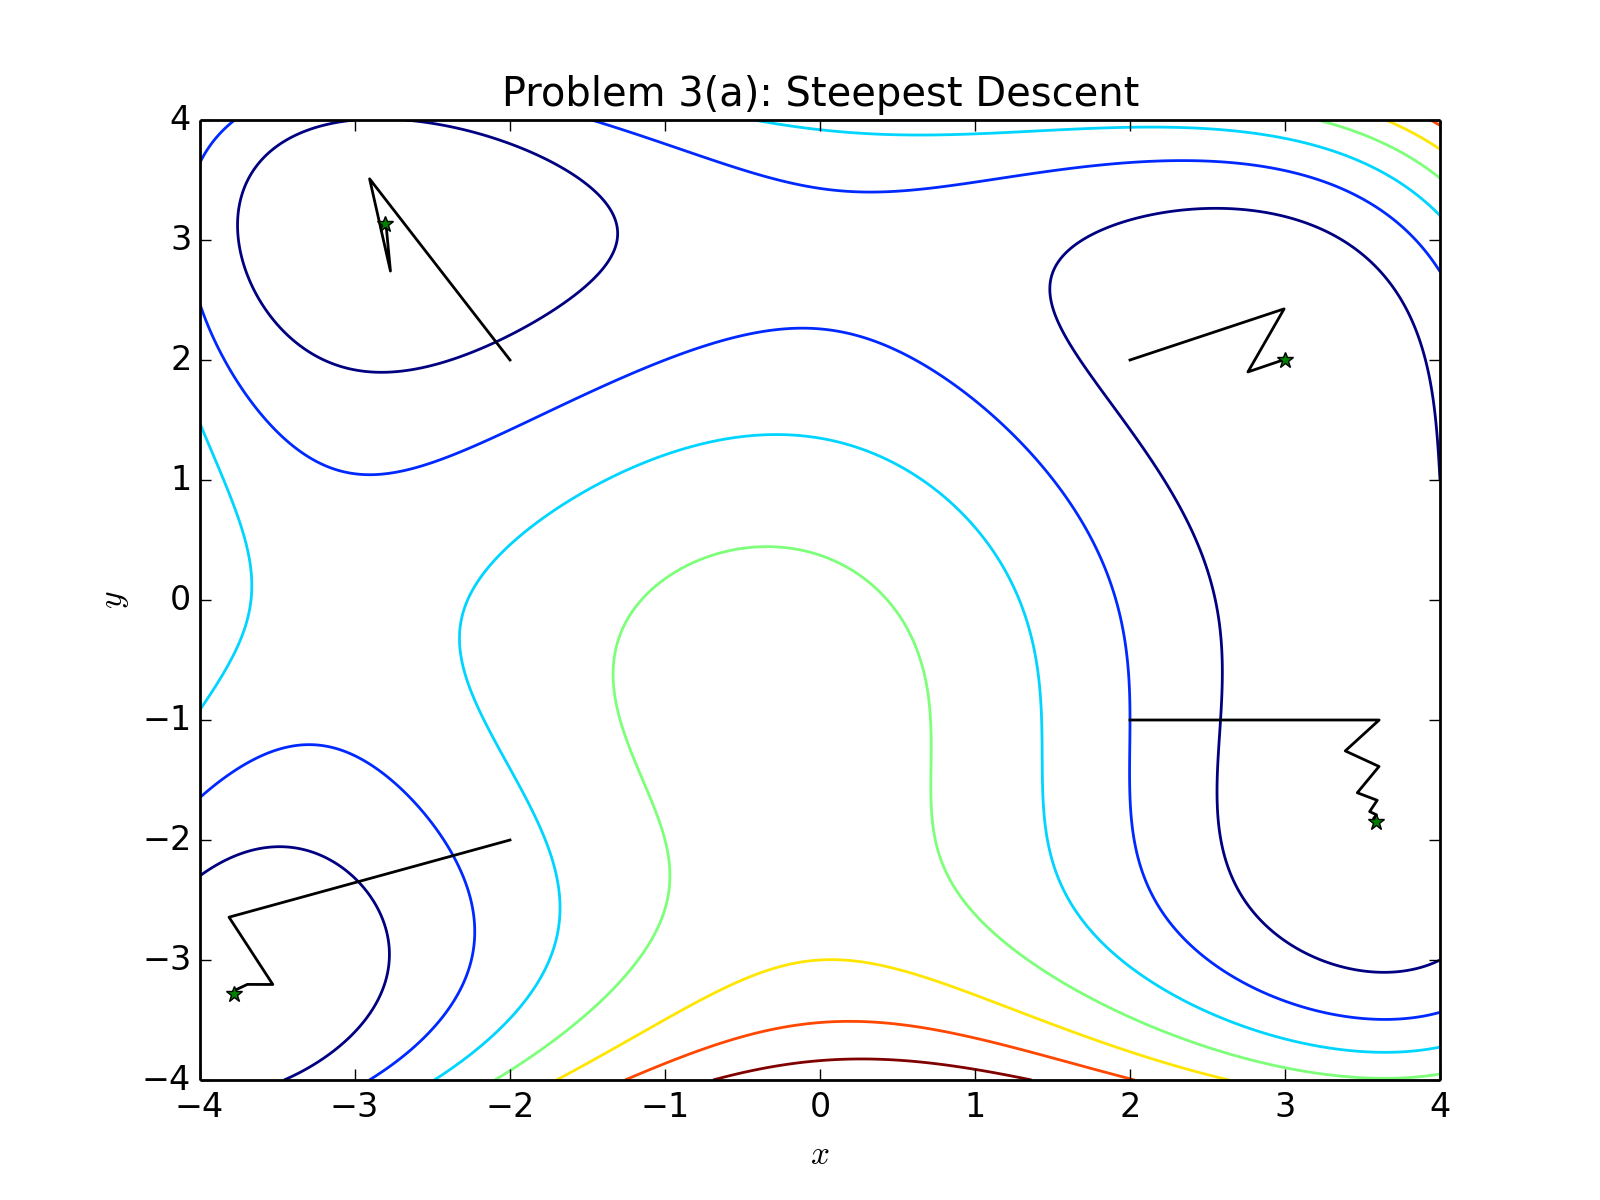
\includegraphics[scale=0.9]{p3afig1}
\end{figure}

\begin{figure}[H]
  \centering
    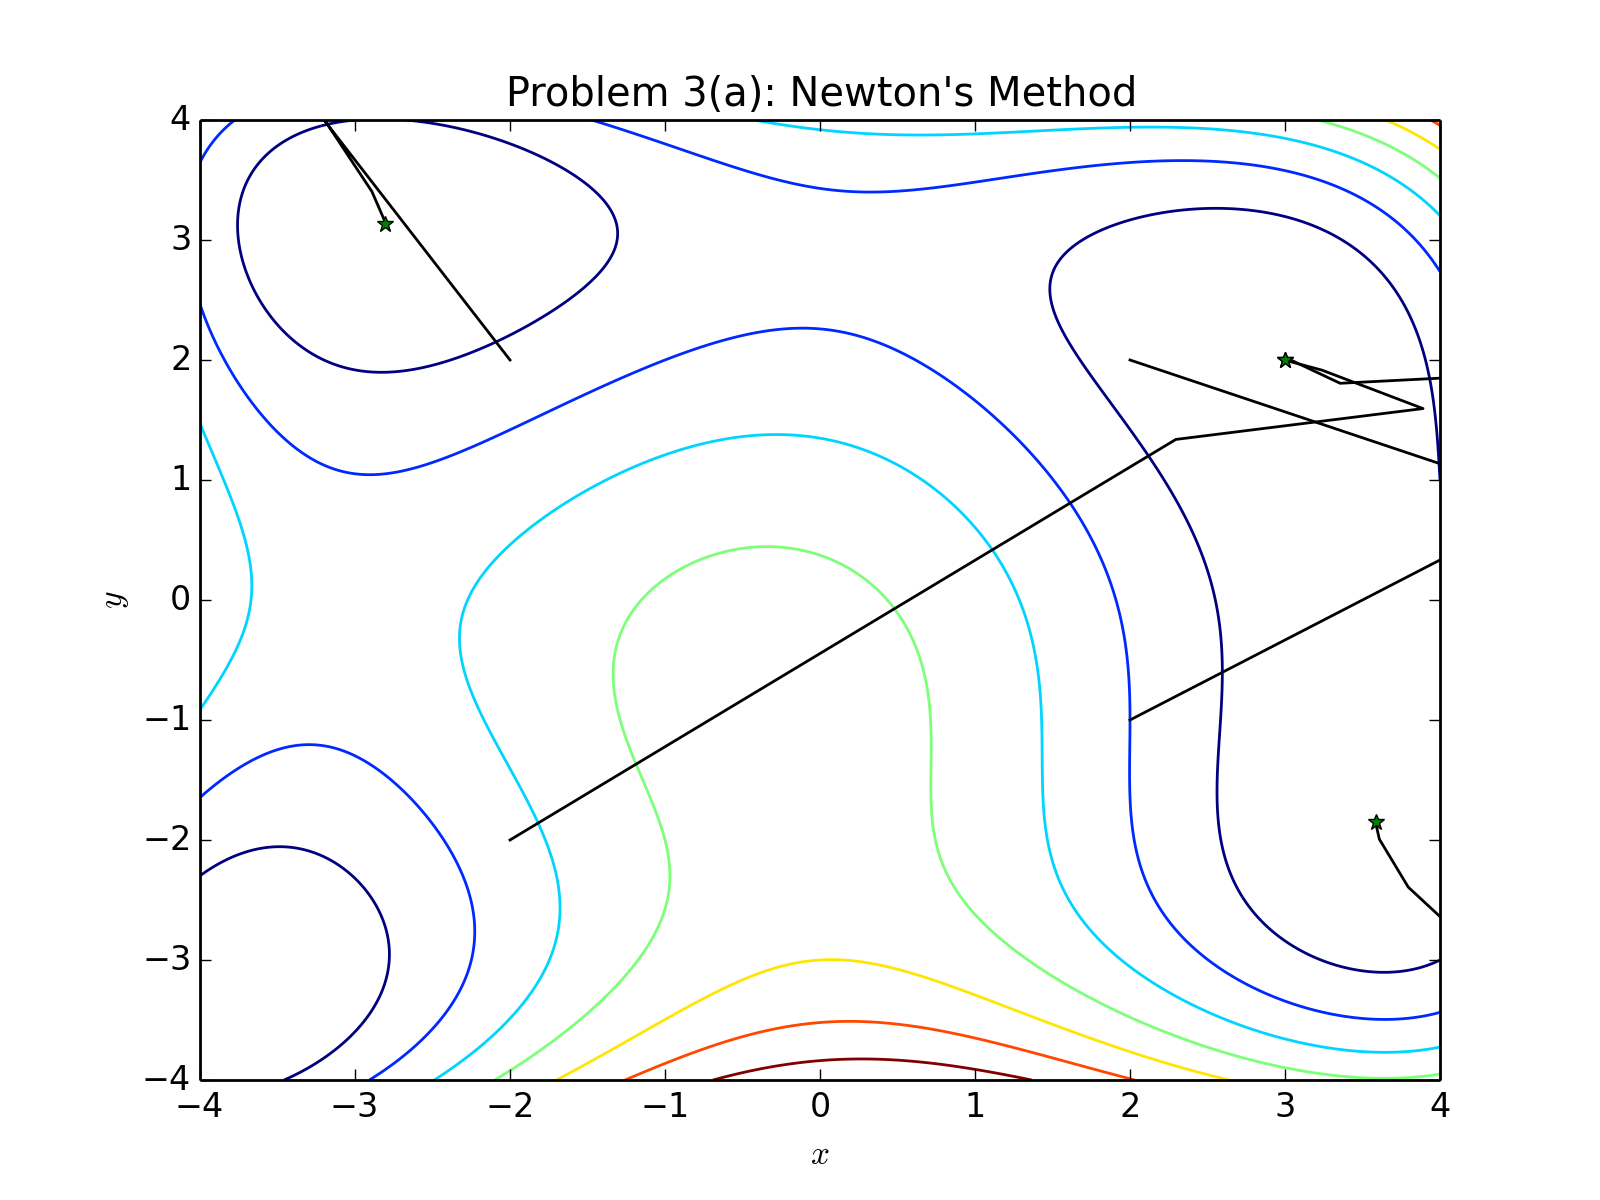
\includegraphics[scale=0.9]{p3afig2}
\end{figure}

\begin{figure}[H]
  \centering
    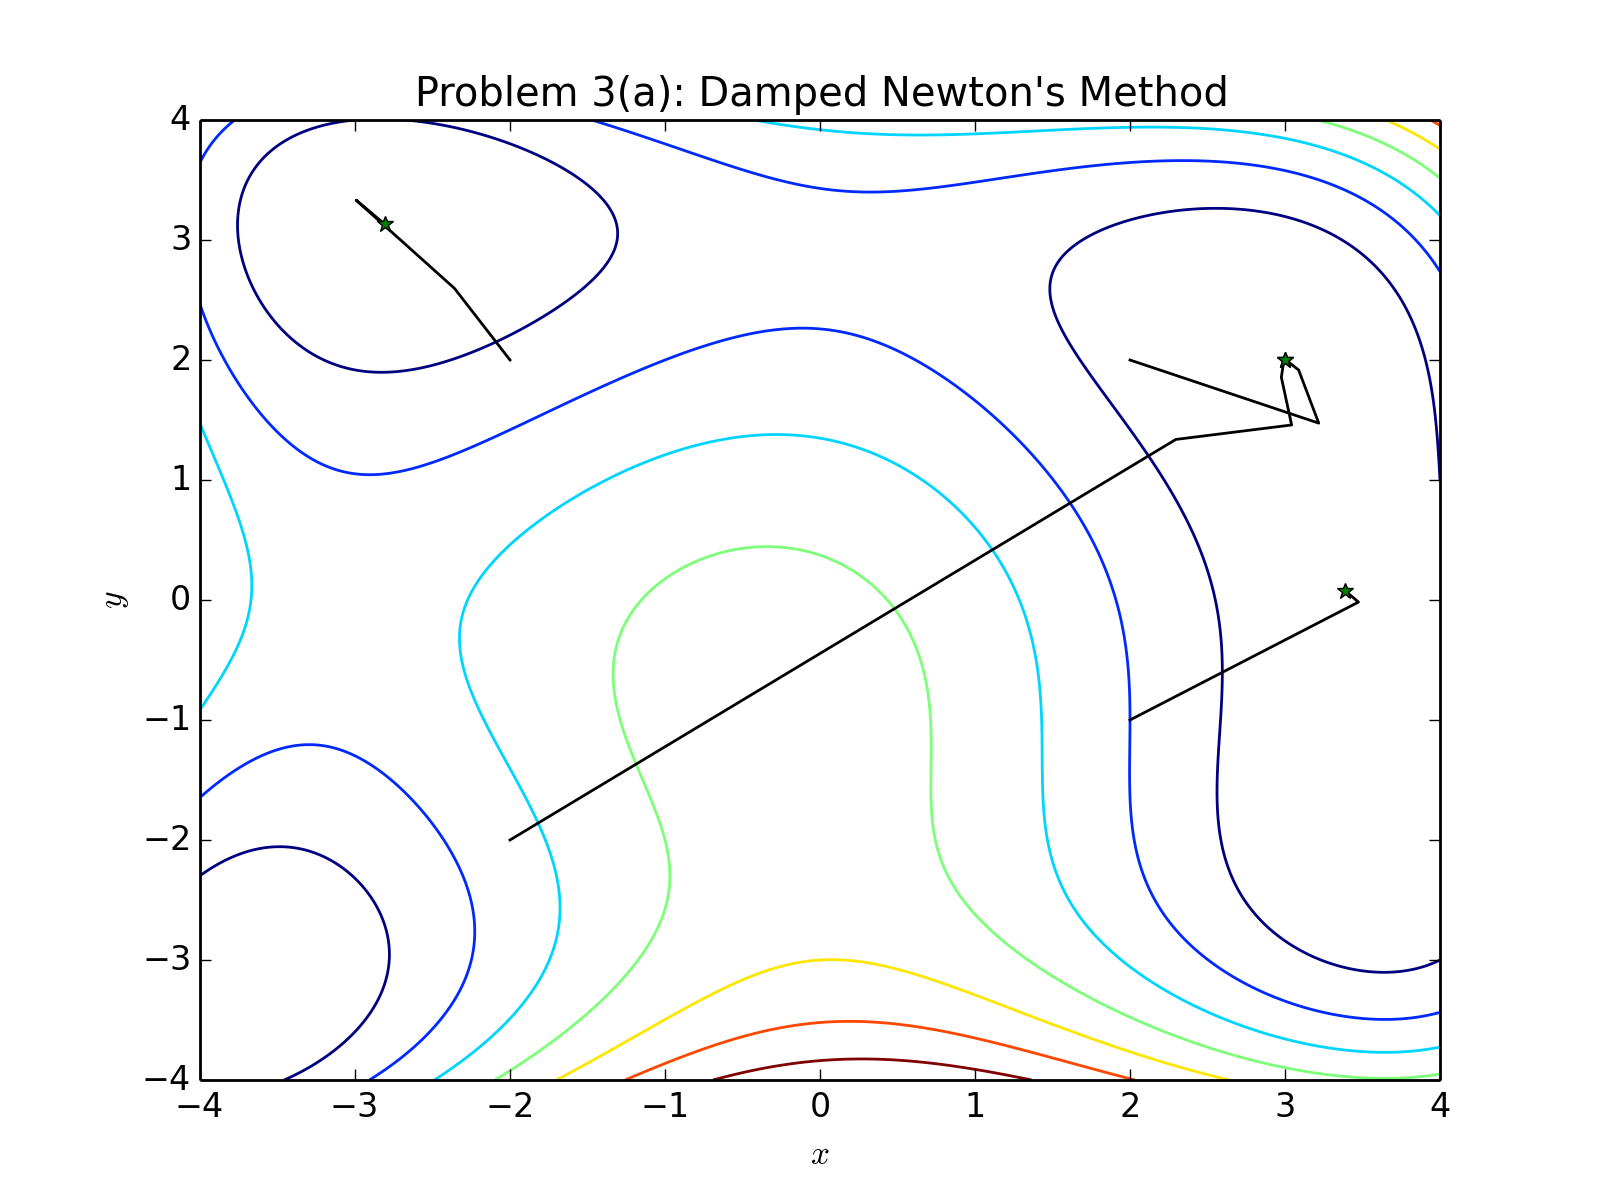
\includegraphics[scale=0.9]{p3afig3}
\end{figure}

\newpage

\item[(b)] See \verb+cs450hw4p3.py+ for my code. The result from the first starting vector matches almost perfectly, the second one is slightly off but still a good fit, and the third is not a good fit at all. The algorithm terminated for each starting vector. Here are the plots for the three cases:

\begin{figure}[H]
  \centering
    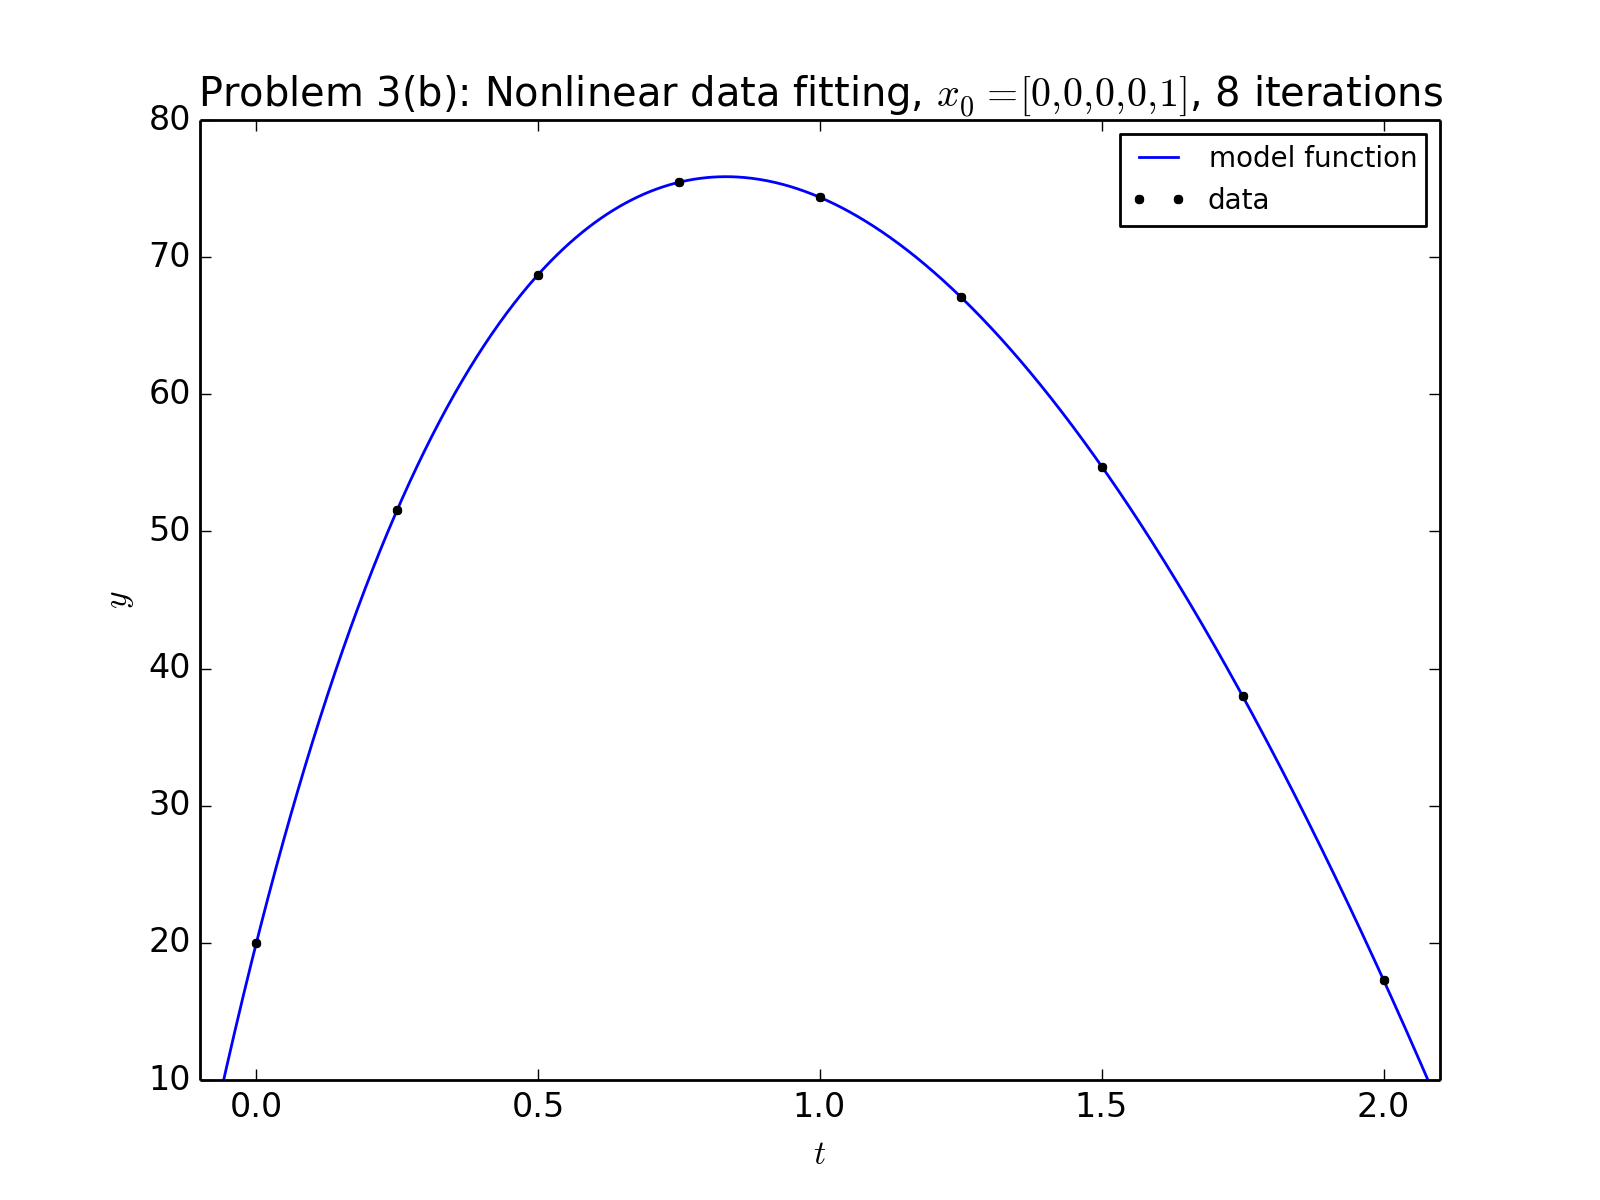
\includegraphics[scale=0.9]{p3bfig1}
\end{figure}

\begin{figure}[H]
  \centering
    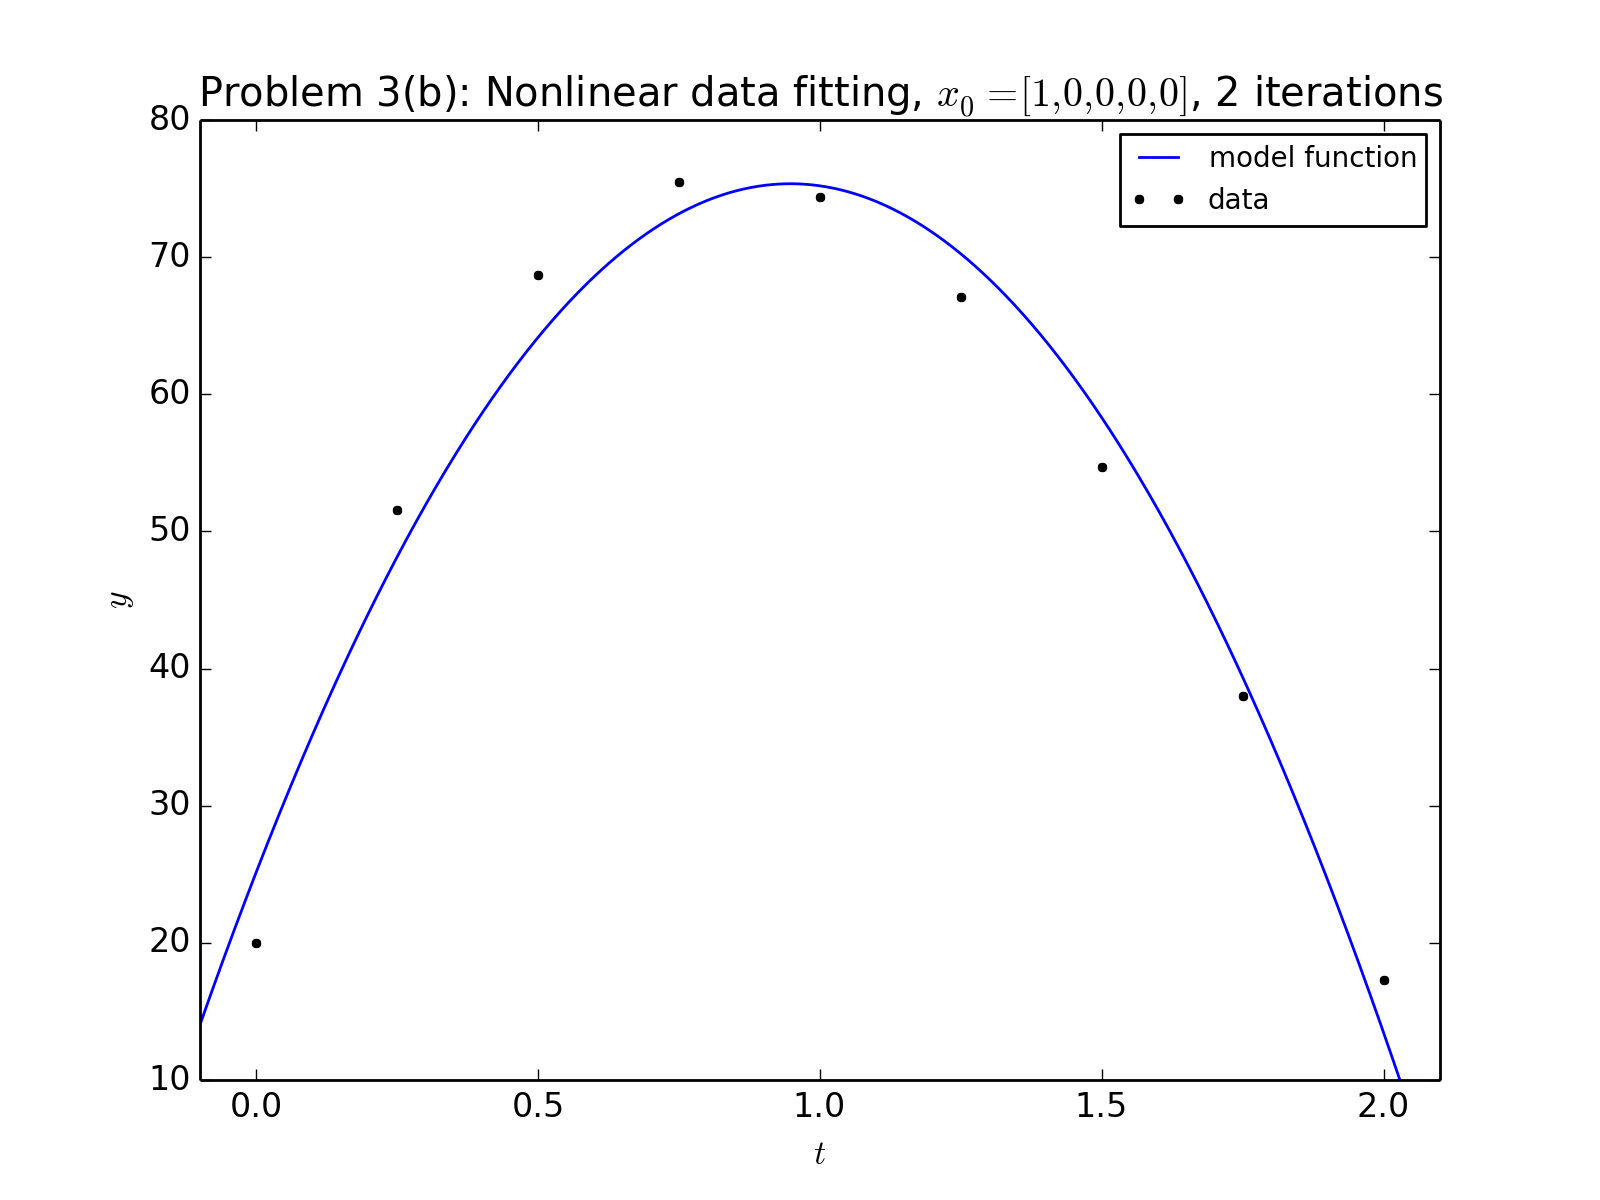
\includegraphics[scale=0.9]{p3bfig2}
\end{figure}

\begin{figure}[H]
  \centering
    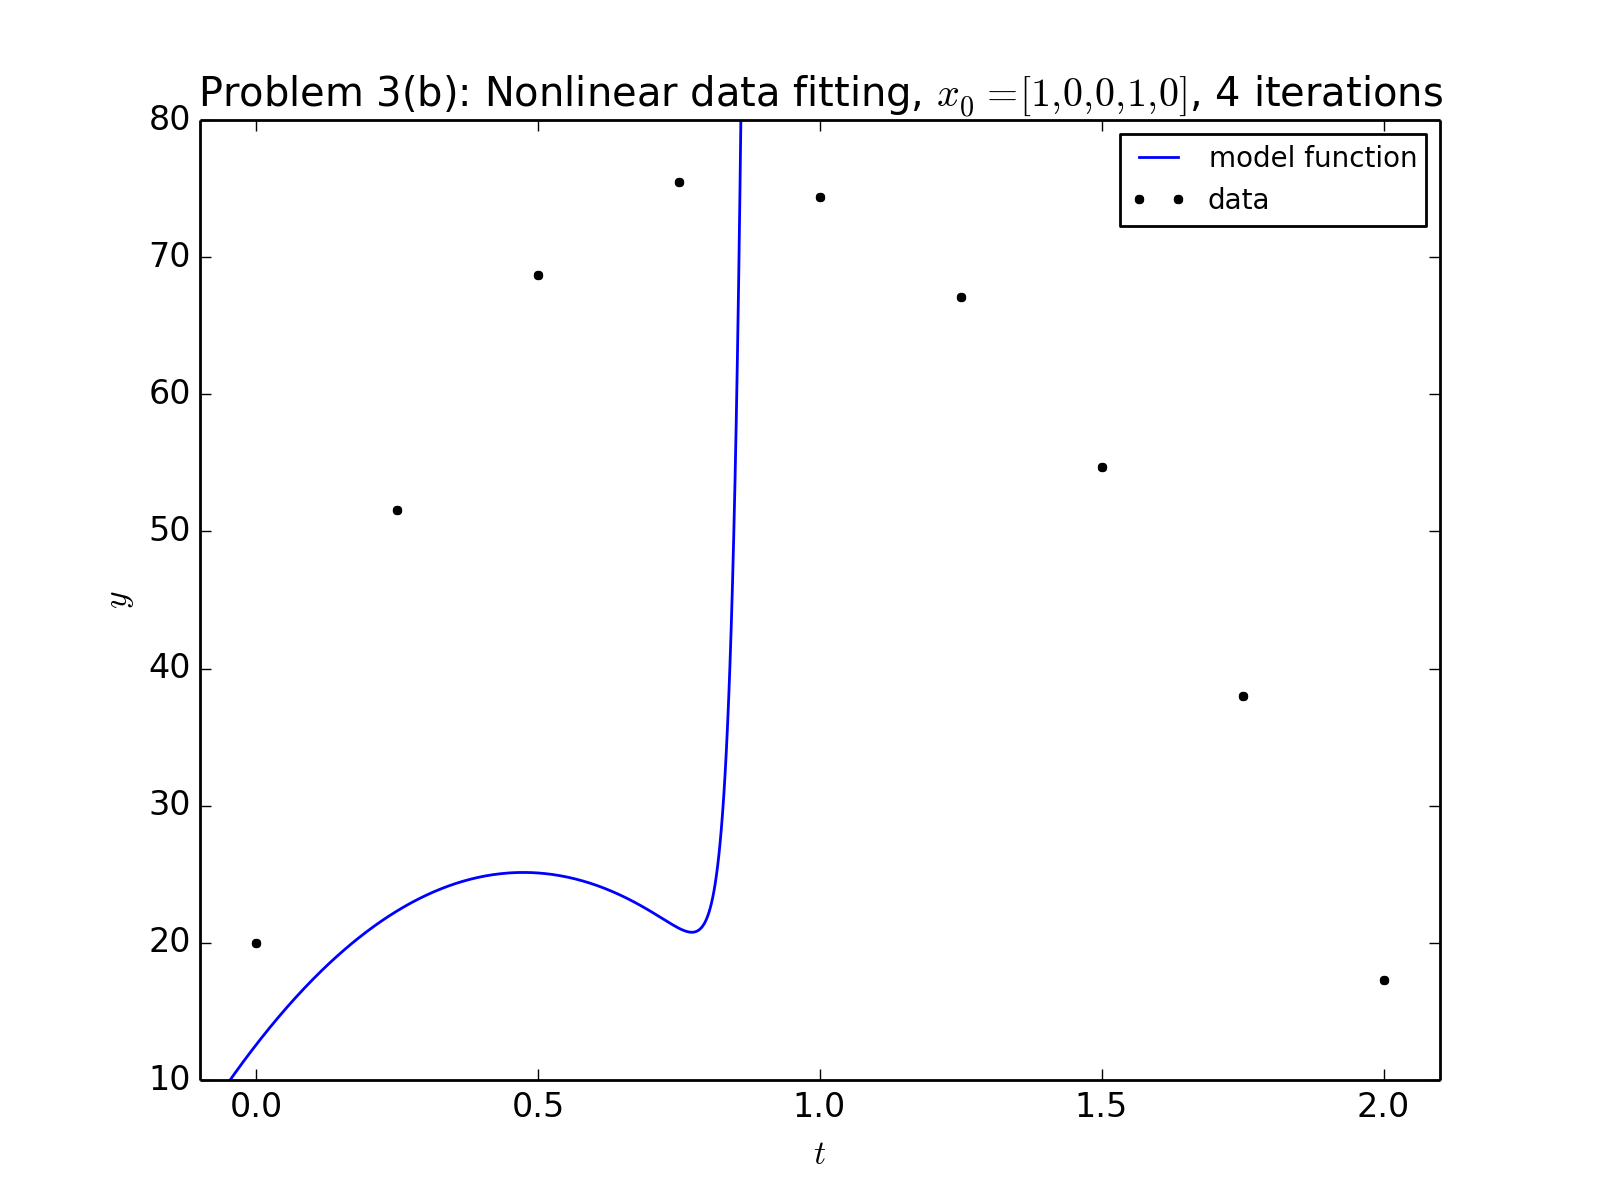
\includegraphics[scale=0.9]{p3bfig3}
\end{figure}

\end{itemize}

\akteachprobhead{%
  Problem 4: Stability of Interpolation (20 points)
}

See \verb+cs450hw4p5.py+ for my code. Runge's phenomenon is when interpolated polynomials blow up near the endpoints of an interval when using equispaced nodes. Chebyshev nodes and Guass-Legendre nodes concentrate near the endpoints to control Runge's phenomenon. Here is my plot:

\begin{figure}[H]
  \centering
    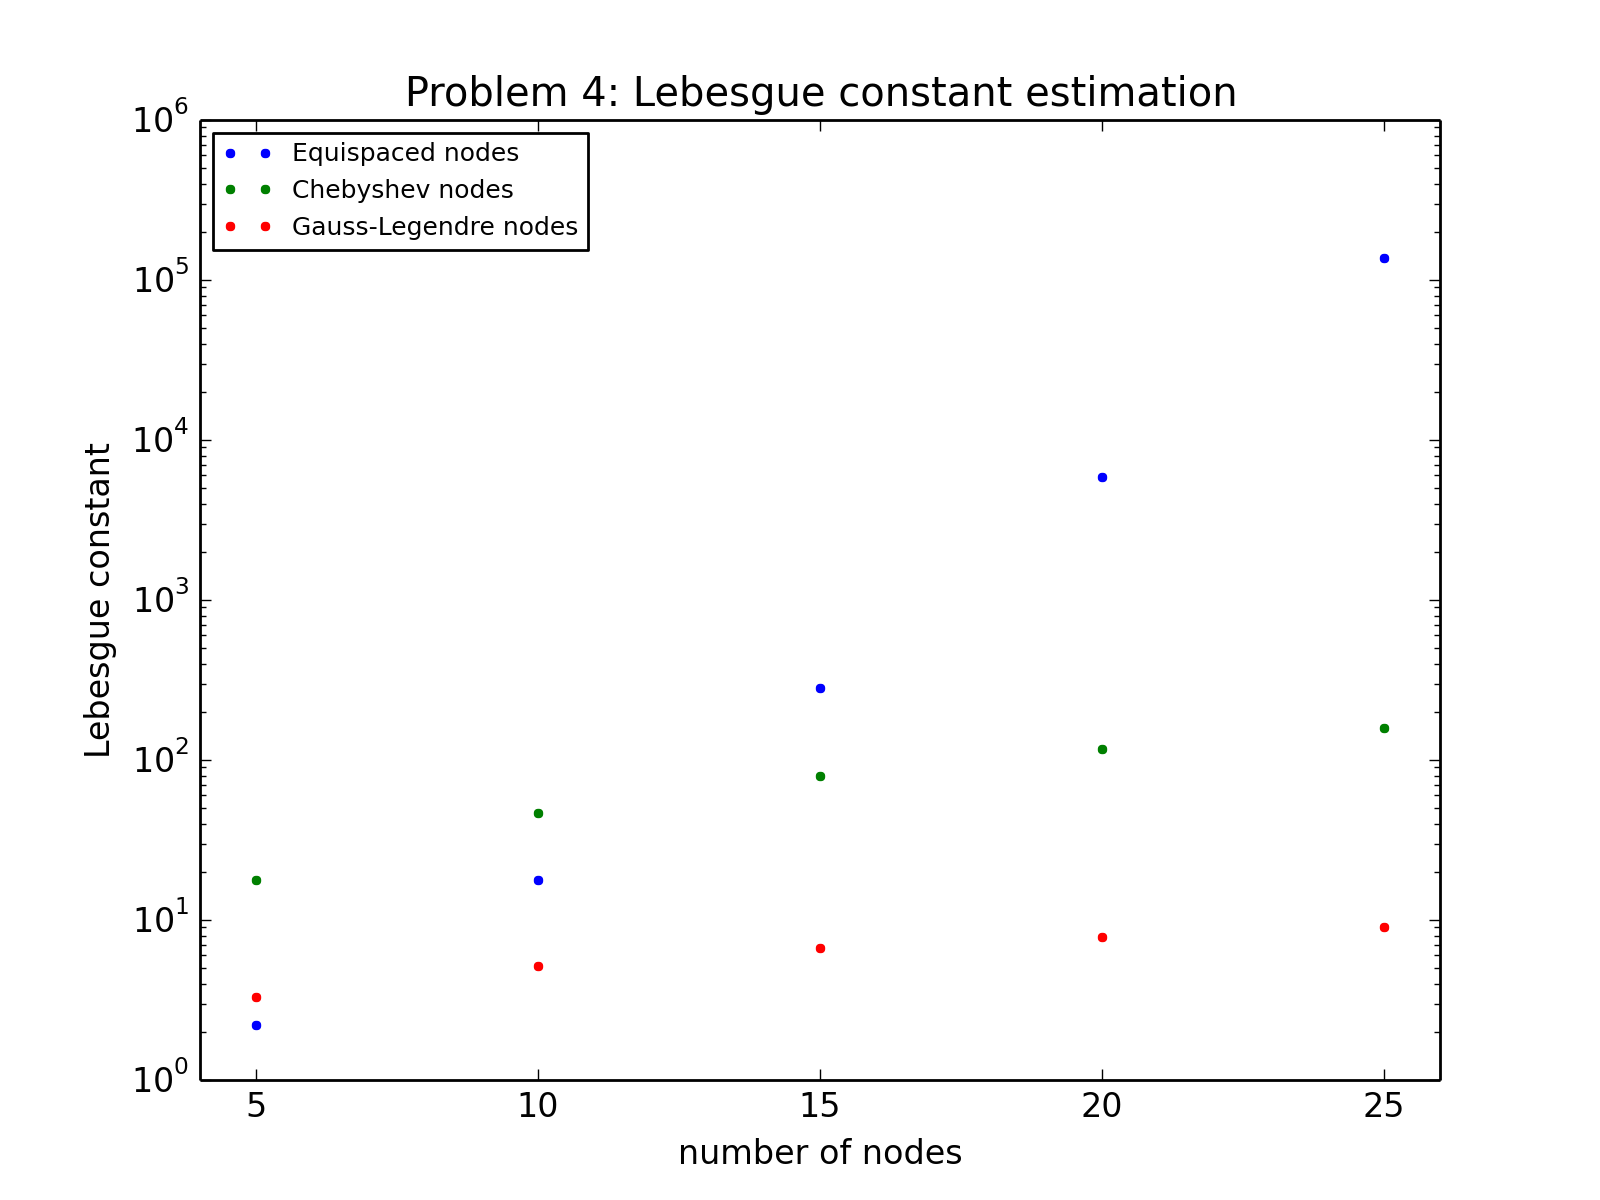
\includegraphics[scale=0.9]{p4}
\end{figure}

\newpage

\akteachprobhead{%
  Problem 5: Chebyshev polynomials, Vandermonde matrices (20 points)
}

\begin{itemize}
\item[(a)] \begin{proof}
Since $ F_n(t) = \cos(n \arccos(t)) $, we clearly have $ F_0(t) = 1 $ and $ F_1(t) = t $. Suppose for $ k = 2, ... , n-1 $, we have $$
F_{k+1}(t) = 2 t F_k(t) - F_{k-1}(t).
$$ Then, $$
F_{n+1}(t) = \cos( (n+1) \arccos(t)) = \cos(n \arccos(t)) \cos(\arccos(t)) - \sin(n \arccos(t)) \sin(\arccos(t))
$$ $$
= 2 \cos(n \arccos(t)) \cos(\arccos(t)) - ( \cos(n \arccos(t)) \cos(\arccos(t))  + \sin(n \arccos(t)) \sin(\arccos(t)) )
$$ $$
2t \cos(n \arccos(t)) - \cos((n-1)\arccos(t)) = 2t F_{n}(t) - F_{n-1}(t).
$$ By induction, $ F_{n+1}(t) = 2 t F_n(t) - F_{n-1}(t) $ for $n \geq 2$.
\end{proof}

\item[(b)] \begin{proof} First, $ F_0(t) = 1 $ and $ F_1(t) = t $ are polynomials. Suppose $ F_0(t), F_1(t), ... , F_n(t) $ are polynomials. Then, $ F_{n+1}(t) = 2 t F_n(t) - F_{n-1}(t) $ is also a polynomial since $ F_n $ and $ F_{n-1} $ are polynomials. By induction $F_n(t)$ is a polynomial for all $n$. \end{proof}

\item[(c)] See \verb+cs450hw4p5.py+ for my code. Here is my plot:

\begin{figure}[H]
  \centering
    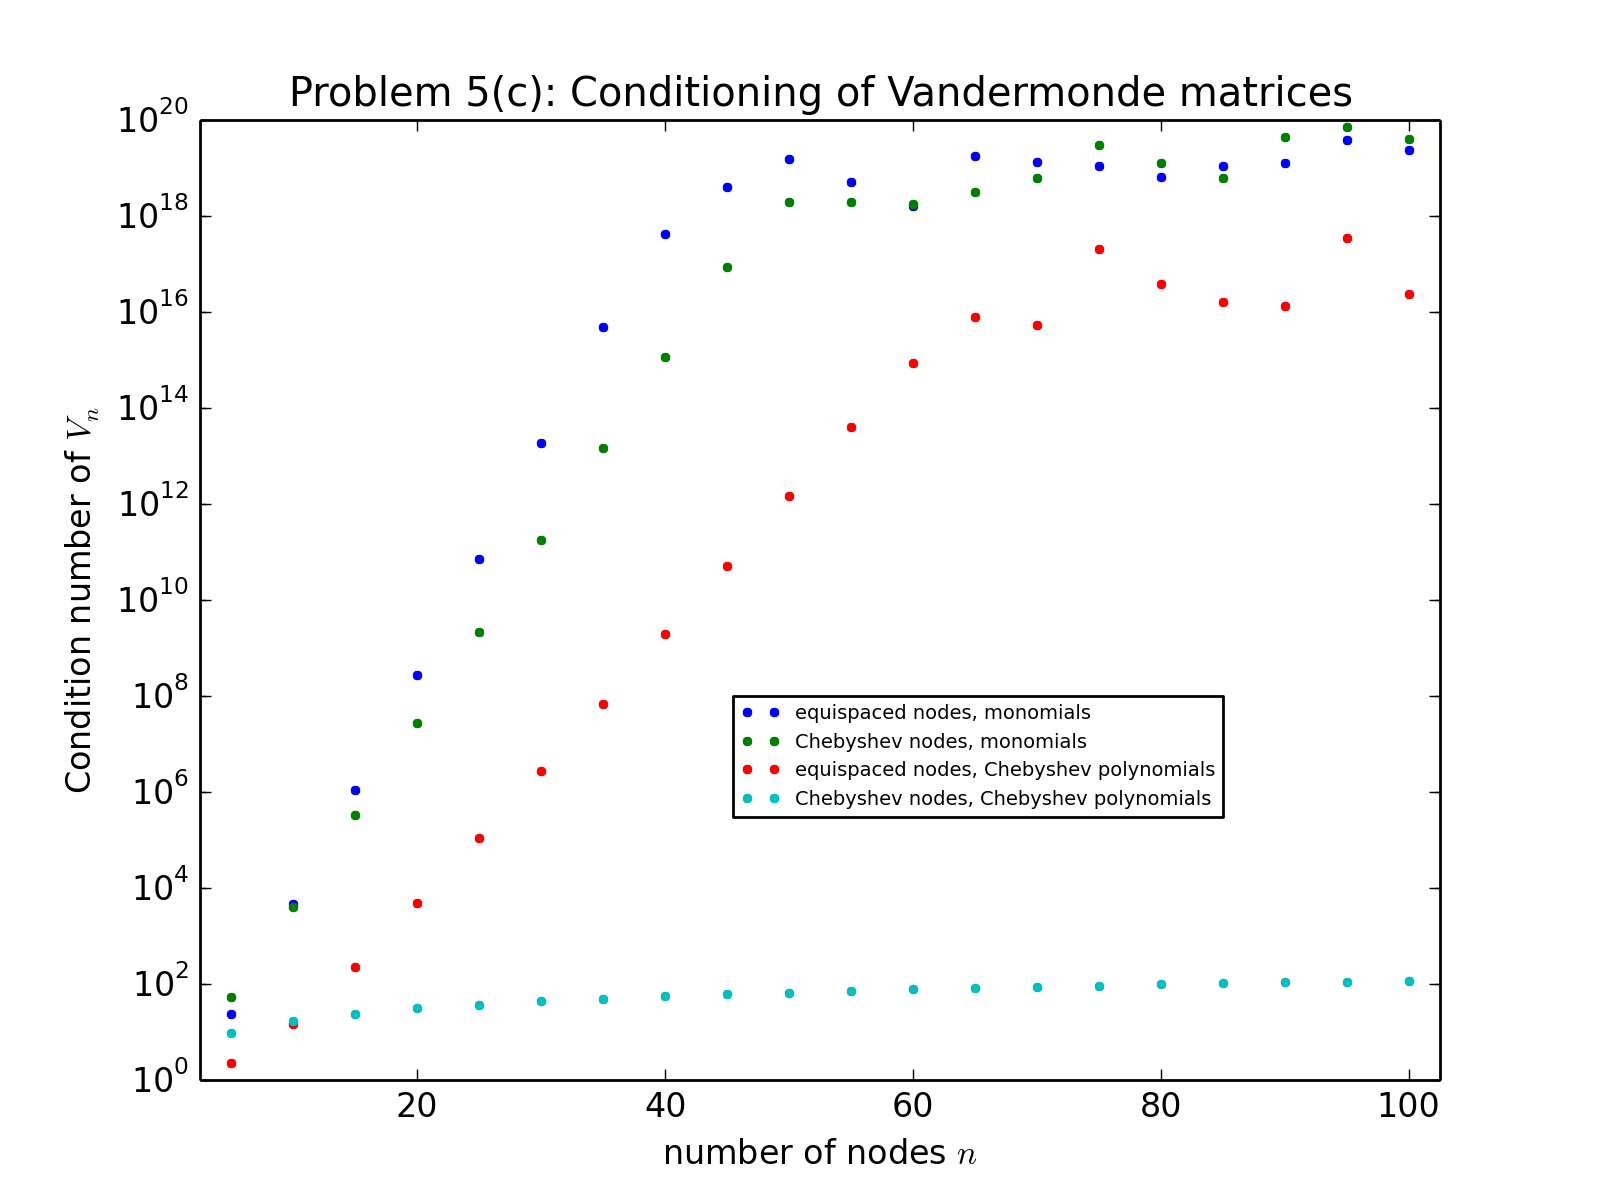
\includegraphics[scale=0.9]{p5}
\end{figure}

\item[(d)] The combination of Chebyshev nodes and Chebyshev polynomials worked best.

\end{itemize}

\end{document}
